The implemented solution of the visualization tool is based on three linked tableau dashboards. Each of these dashboards consists of several workbooks, which are linked functionally by so-called actions. Each workbook of the dashboard provides subtasks for the fulfilment of the main tasks of one dashboard. Fig~\ref{fig:overviewdashboard} shows the user interface of all the three created dashboards.

\begin{figure}[ht]
   \begin{minipage}[b]{.5\linewidth}          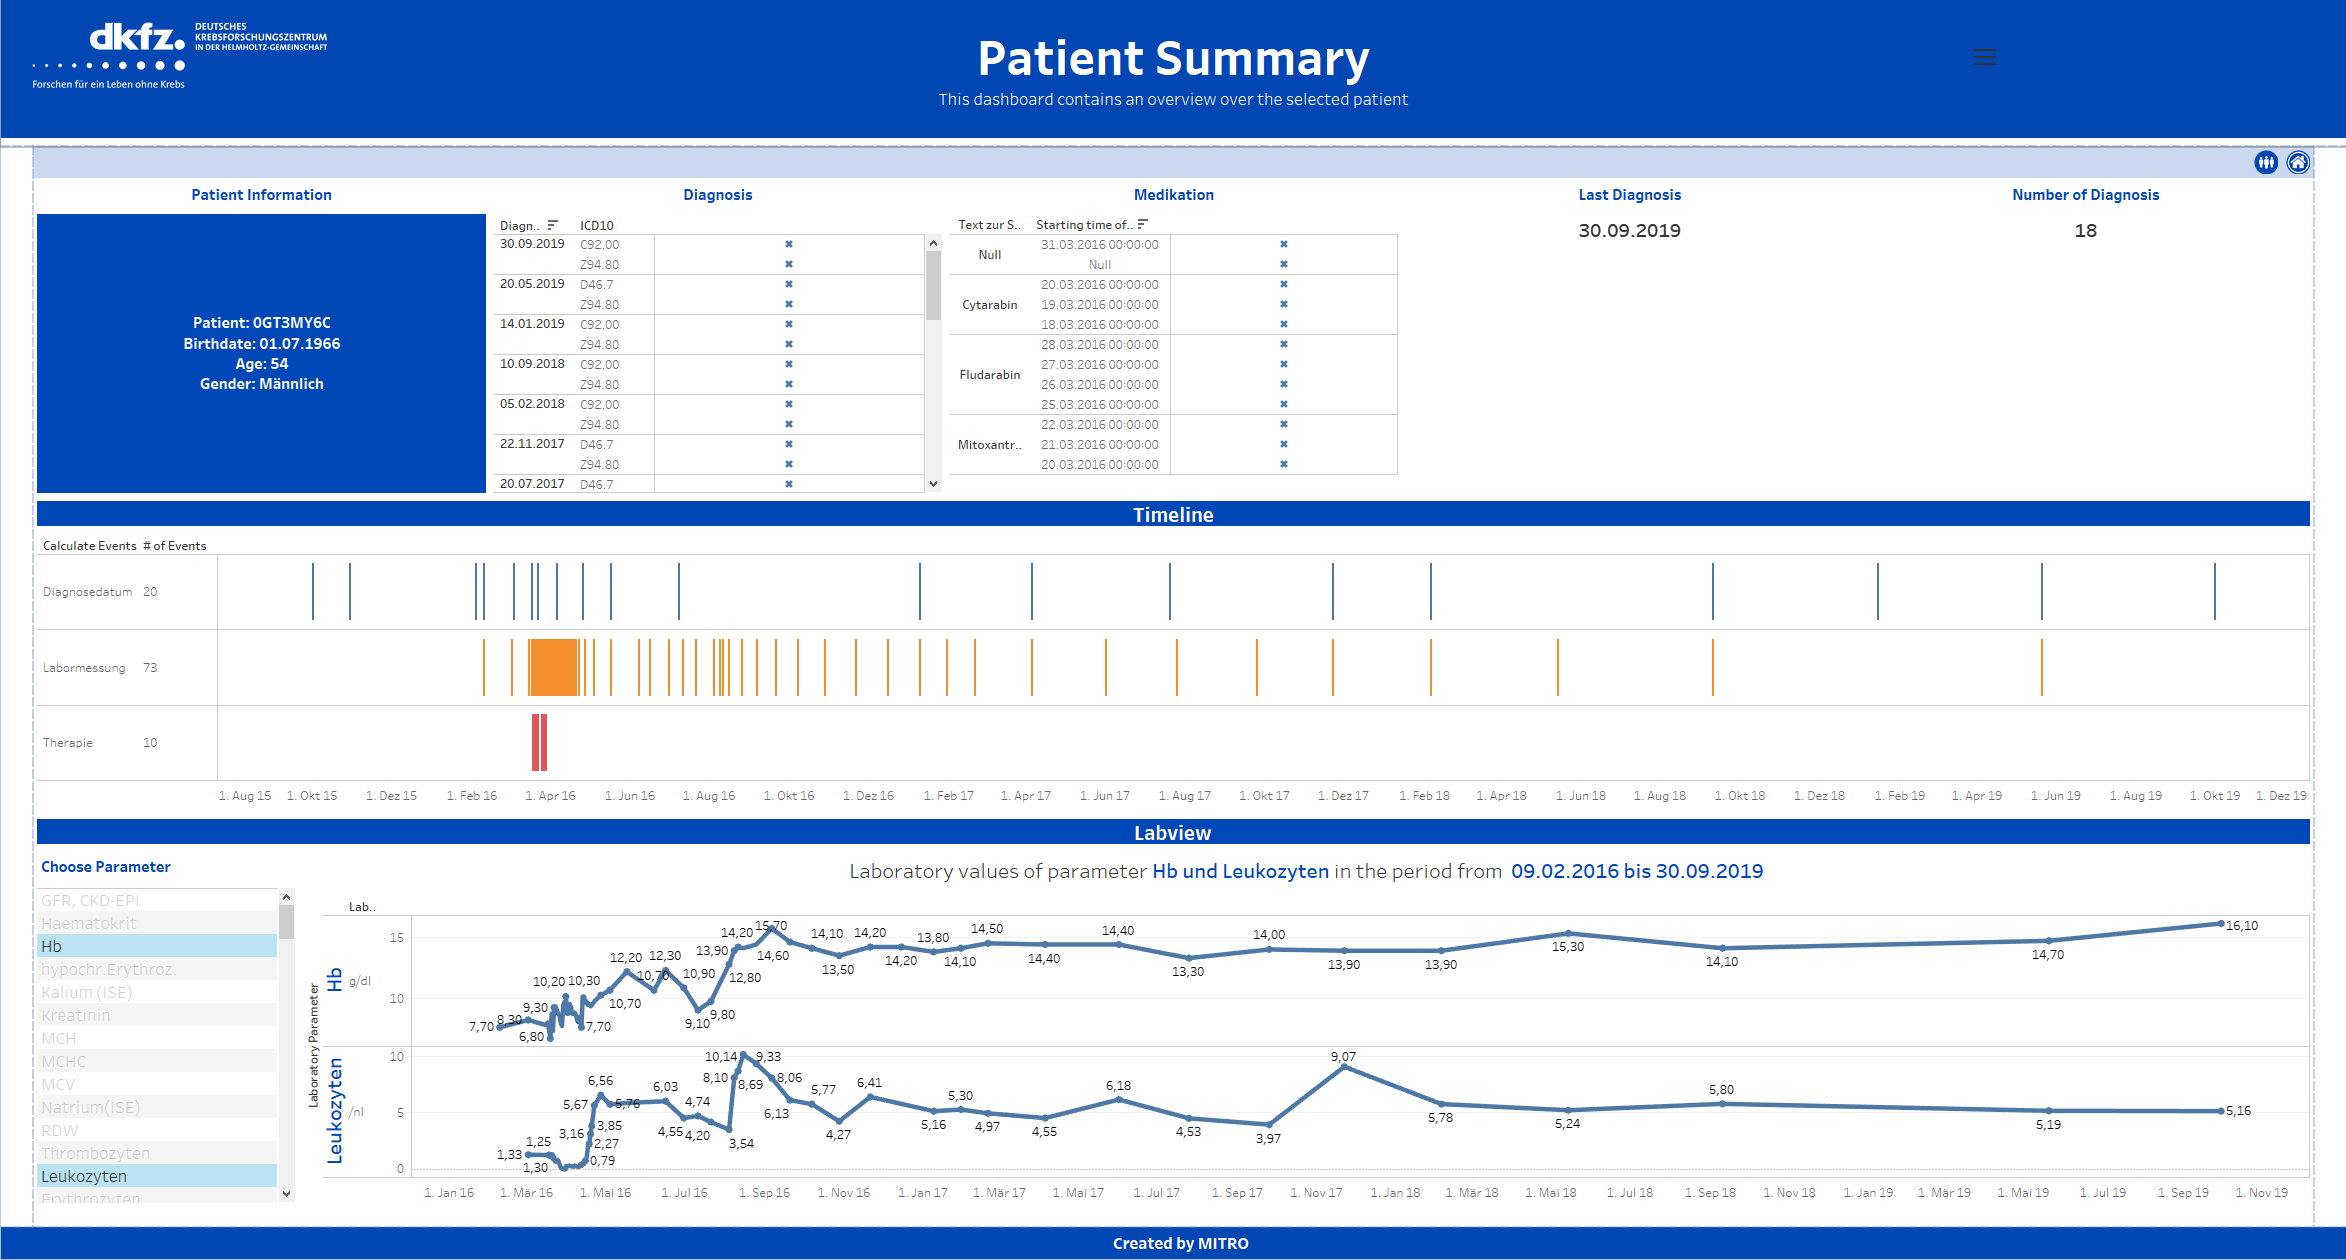
\includegraphics[width=1.05\textwidth]{images/Pat sum.png}
   \end{minipage}% 
   \hfill
   \begin{minipage}[b]{.5\linewidth} 
 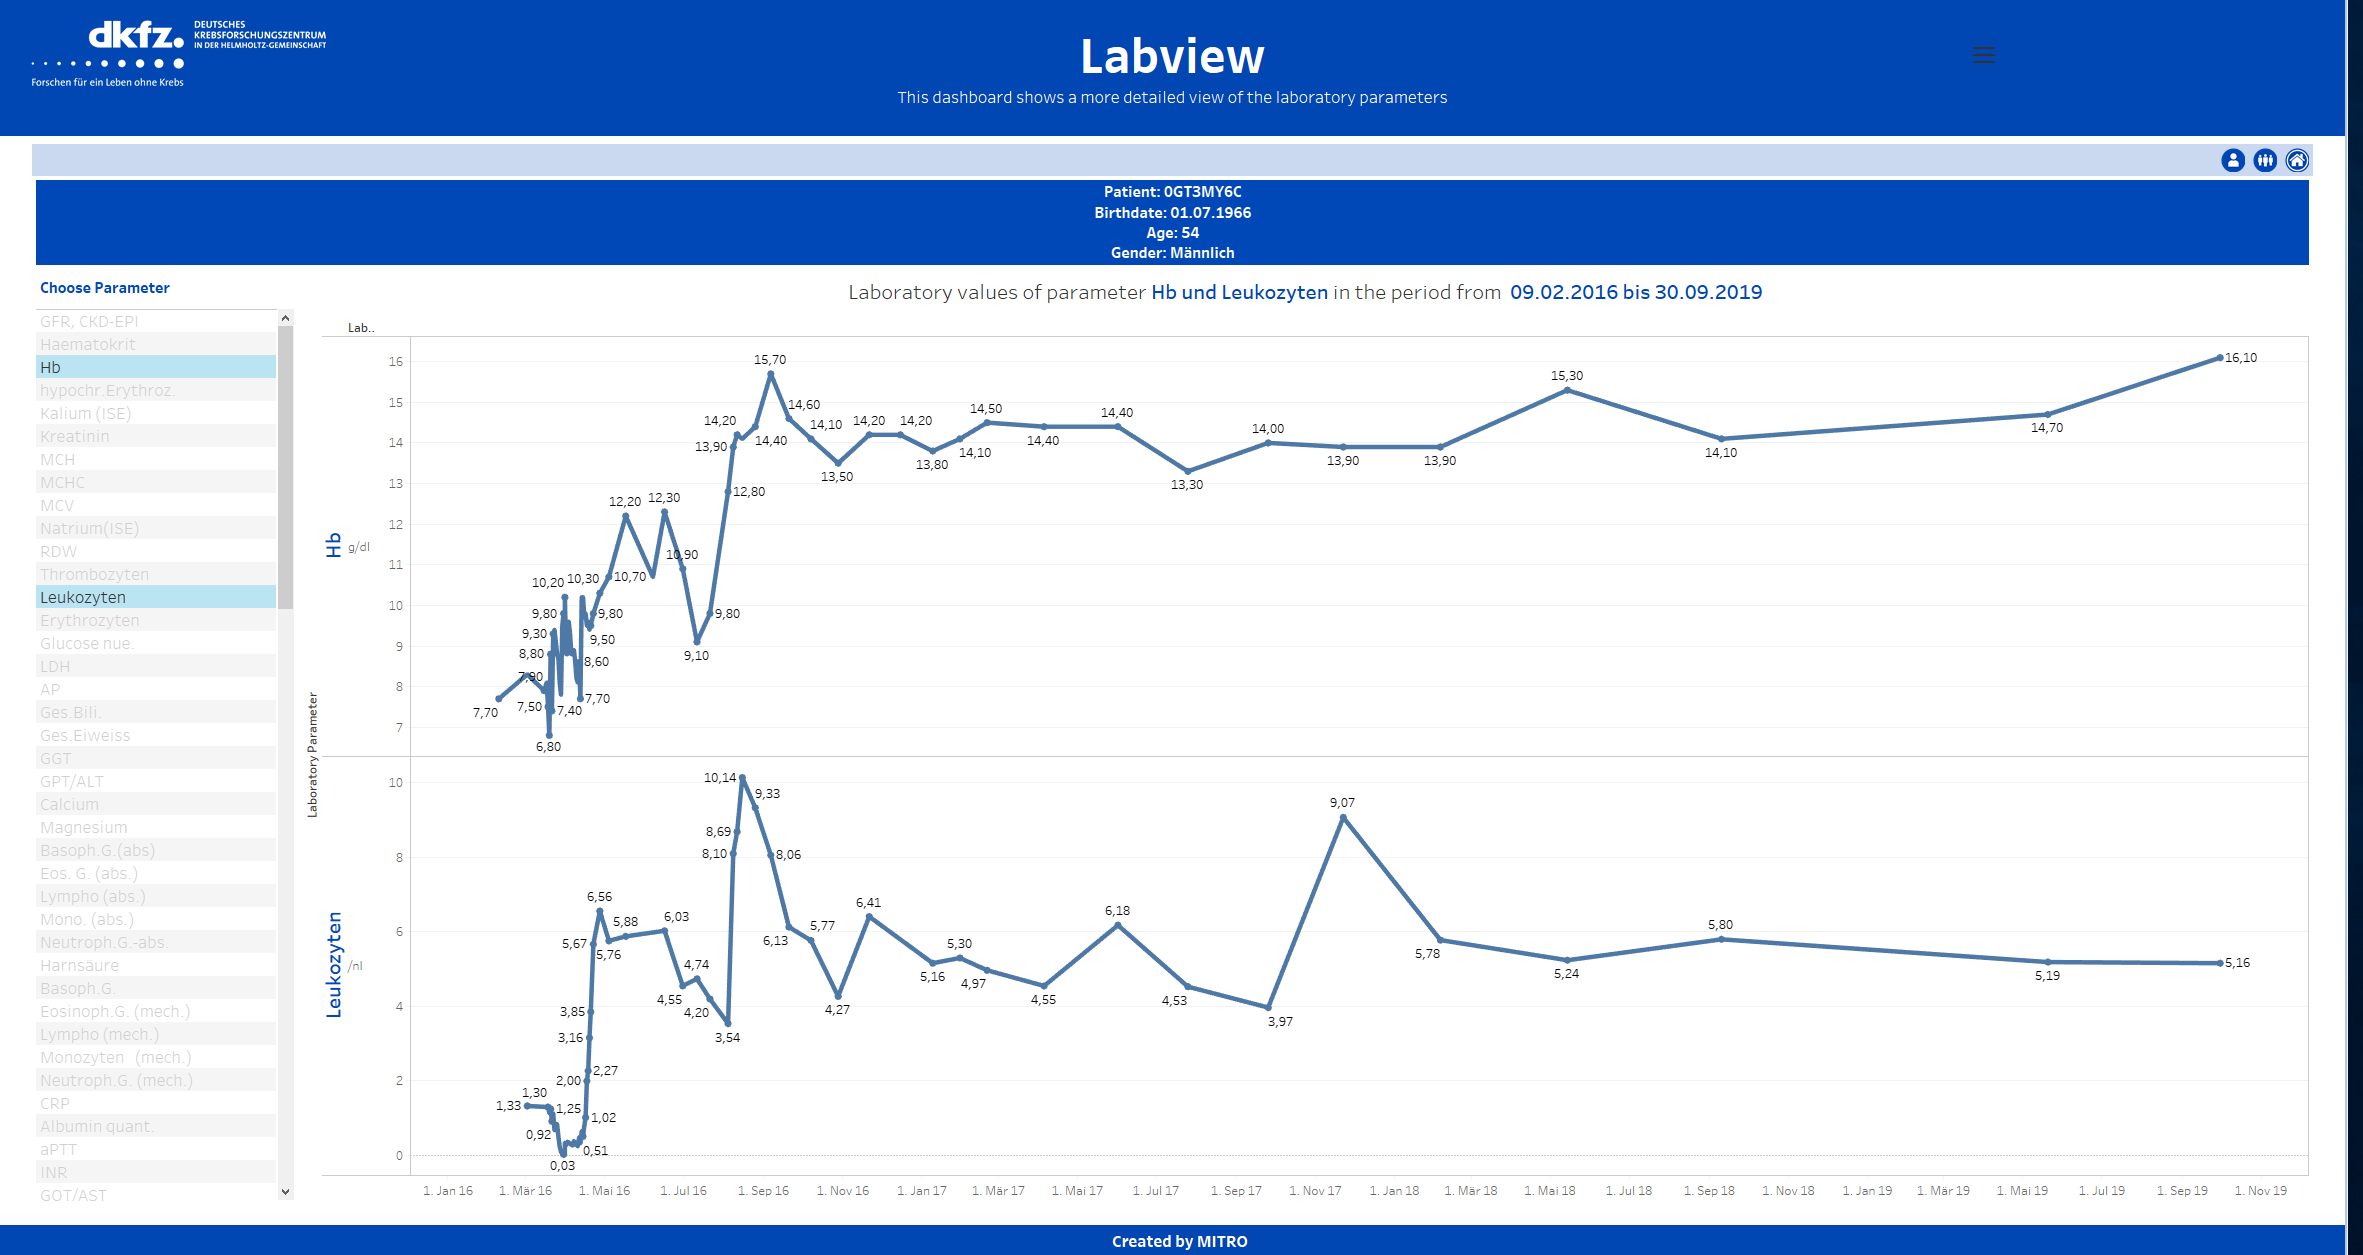
\includegraphics[width=1.05\textwidth]{images/Labview.png} 
   \end{minipage}%
   \vfill
      \begin{minipage}[b]{\linewidth}          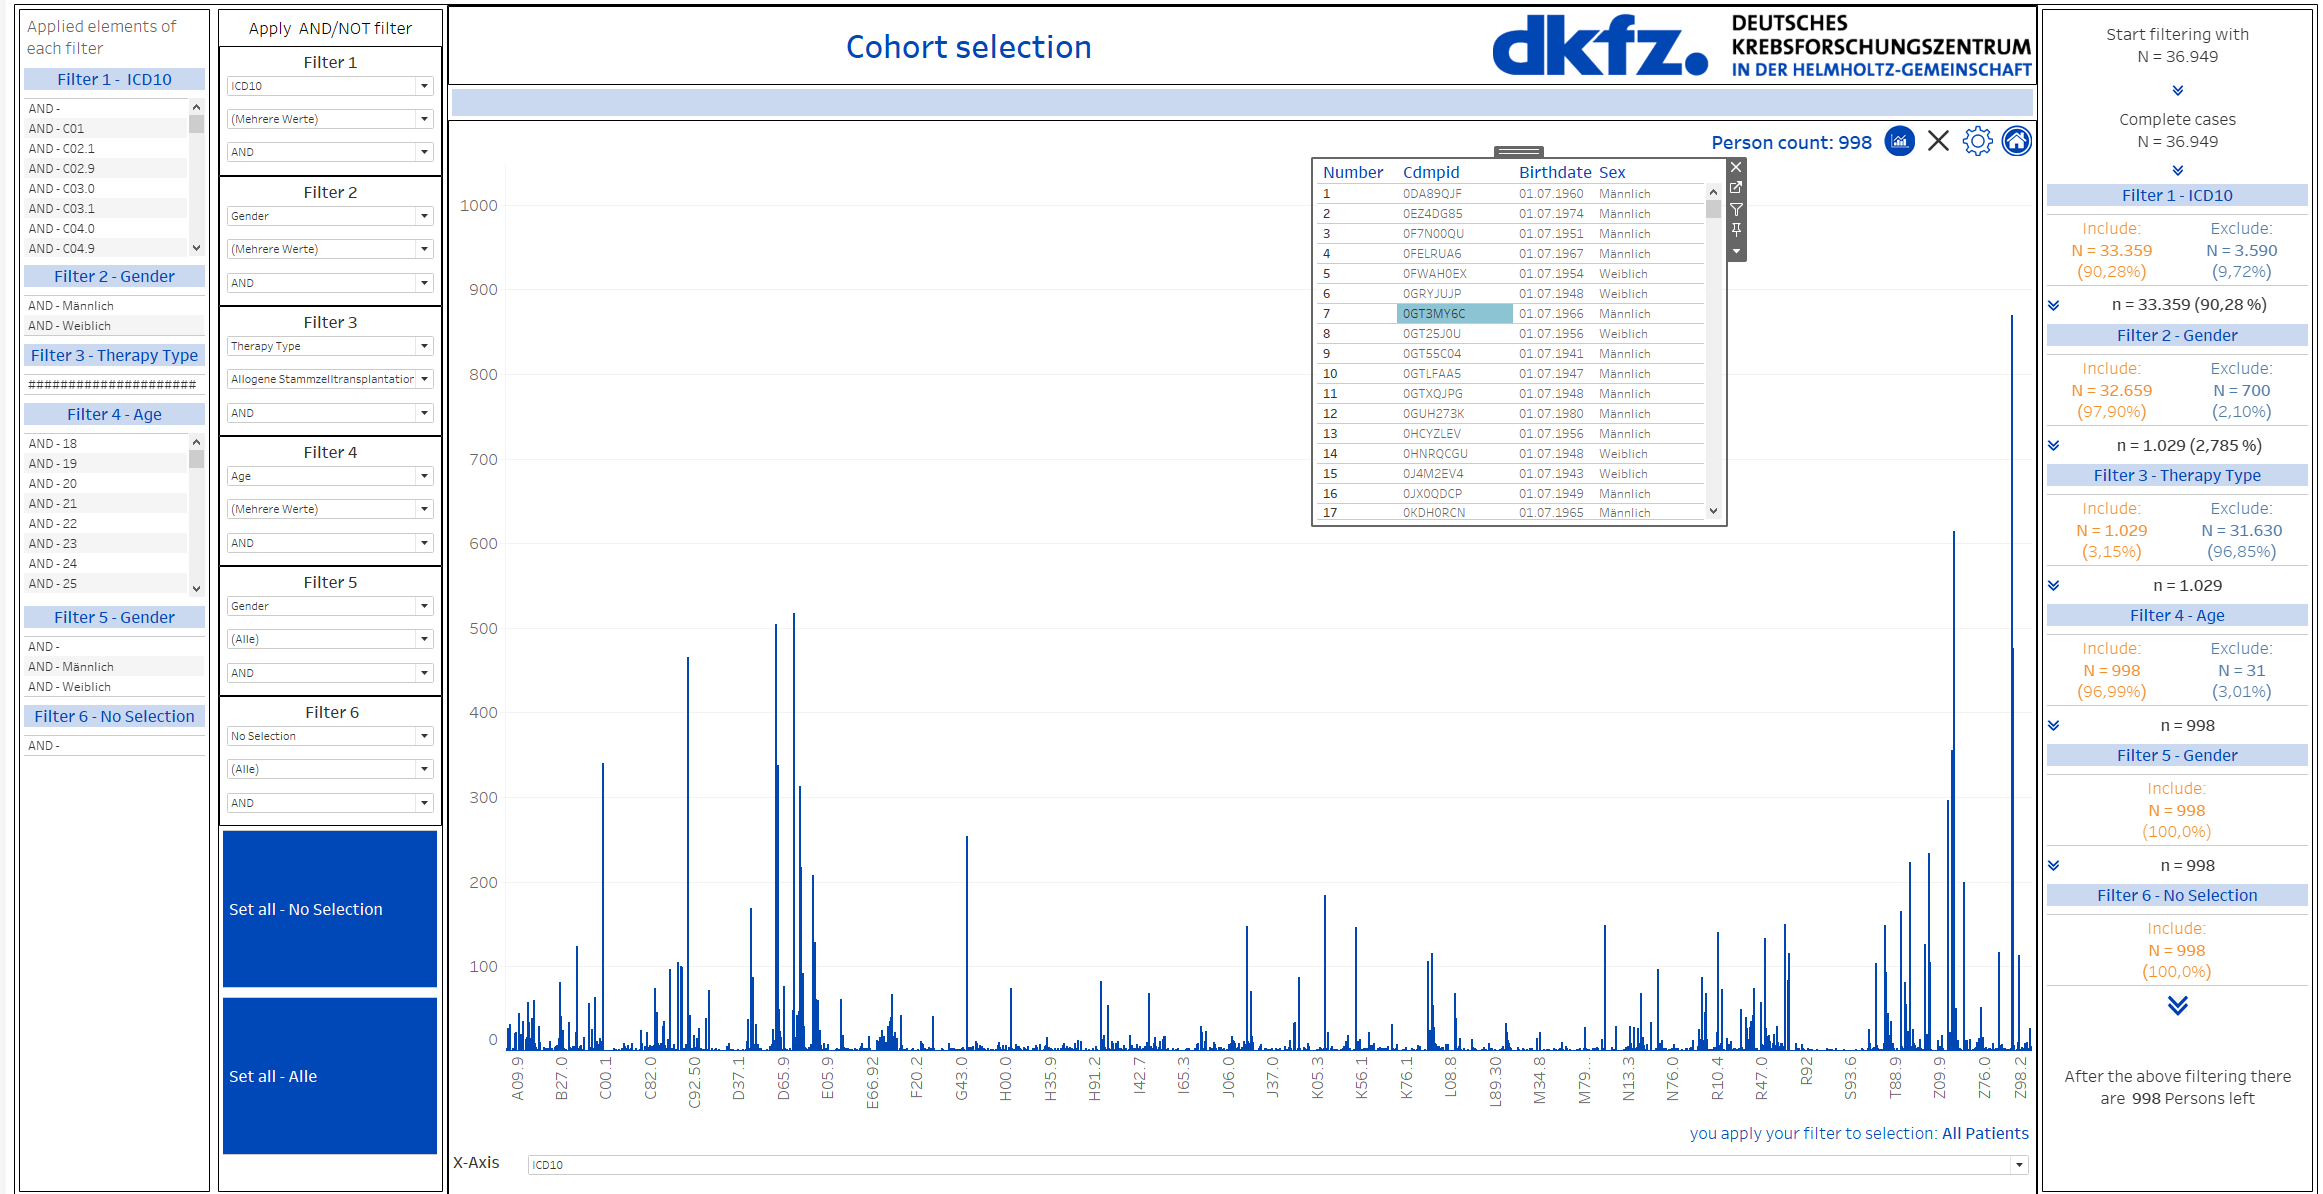
\includegraphics[width=1.05\textwidth]{images/ch sel.png}
   \end{minipage}% 
   \caption{User Interface of the three implemented dashboards}\label{fig:overviewdashboard} 
\end{figure} 

The Patient summary dashboard contains three main components. The top part contains information of the selected patient and displays variables like birthday, age, religion, eth